\section{Redes de Sensores Sem Fio}

Redes de sensores sem fio (RSSF) são redes compostas por um grande número de nós sensores densamente distribuídos dentro de um fenômeno ou próximo a ele, cujas posições não precisam ser predeterminadas e que trabalham de forma cooperativa para a realização de tarefas. Isso possibilita a distribuição aleatória em regiões inacessíveis, porém também torna necessária a criação de protocolos e algoritmos com capacidade de auto organização\cite{Akyildiz2002}.

\citeauthoronline{Romer2004} (\citeyear{Romer2004}) definem RSSF como redes \textit{ad hoc} de larga escala, \textit{multi-hop}, não particionada composta por nós sensores, em sua maioria imóveis, largamente homogêneos, pequenos e com recursos limitados, randomicamente distribuídos em uma área de interesse.

%%%%%%%%%%%%%%%%%%%%%%%%%%Graças aos crescentes avanços tecnológicos na área de comunicação sem fio e de eletrônicos, tem sido cada vez mais fácil desenvolver nós sensores multifuncionais de baixo custo e consumo de energia capazes de se comunicar a curtas distâncias. Isso vem alavancado e tornando viável a utilização desse tipo de rede para os mais diversos tipos de aplicações.

\begin{figure}[!htb]
\centering
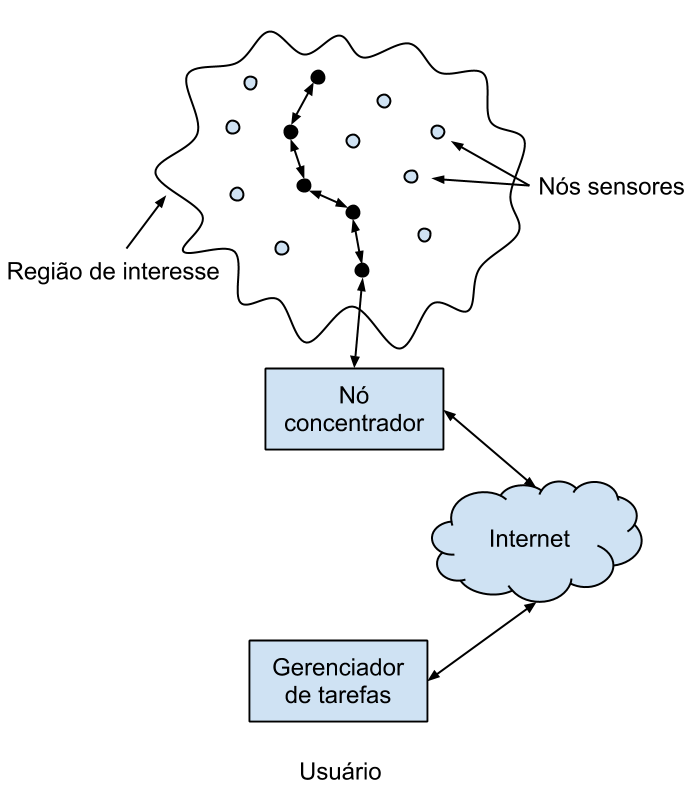
\includegraphics[width=200px,height=280px]{./Pictures/SensorNodesScatteredInASensorField.png}
% SensorNodesScatteredInASensorField.png: 816x1056 pixel, 96dpi, 21.59x27.94 cm, bb=0 0 612 792
% pdfLaTeX aceita figuras no formato PNG, JPG ou PDF
% figuras vetoriais podem ser exportadas para eps e depois convertidas para pdf usando epstopdf
\caption{Exemplo da distribuição dos nós de uma RSSF em uma região de interesse} %legenda
\label{fig:snsf} %rotulo para refencia
\end{figure}

A Figura~\ref{fig:snsf} mostra um exemplo da disposição de uma rede desse tipo. Nesse exemplo os nós da rede de sensores ficam distribuídos em uma região de interesse (\textit{sensor field}). Cada um dos nós (\textit{sensor nodes}) coleta dados do ambiente e pode roteá-los até o nó \textit{sink} (nó que reúne as informações da rede) e este pode comunicar-se com o gerenciador de tarefas por meio da internet ou de satélites.

\citeauthoronline{Karl2005} (\citeyear{Karl2005}) apresentam uma definição de redes \textit{ad hoc} como redes configuradas para, literalmente, atender a um propósito específico e a necessidades específicas de comunicação. \cite{Karl2005} apresenta também uma definição para \textit{Mobile Ad Hoc Networks} (MANET) que seria uma rede \textit{ad hoc} associada à comunicação sem fio (\textit{wireless}) e à mobilidade dos nós participantes. 


Listadas abixo estão algumas diferenças significativas entre redes \textit{ad hoc} e RSSF:
\begin{itemize} 
	\item O número de nós sensores em RSSF pode ser de uma ordem de magnitude muio acima da encontrada em redes \textit{ad hoc} \cite{Akyildiz2002}.
	\item MANET são utilizadas em aplicações como comunicação por voz ou acesso a infraestrutura remota necessitando assim de equipamentos robustos o suficiente para suportar esse tipo de aplicações ao contrário de RSSFs que são compostas por equipamentos bem mais simples e limitados \cite{Karl2005}. 
	\item RSSF são capazes de comportar variados cenários de aplicação, devido ao grande número de combinações possíveis de tecnologias de comunicação, computação e sensores. Por exemplo conseguindo trabalhar em diversas e variáveis densidades, o que irá requerer o uso de diferentes protocolos ou protocolos adaptativos. Tal flexibilidade existe também em MANET, porém em um nível bastante reduzido \cite{Karl2005}. 
	\item A densidade das RSSF é bem maior que a encontrada nas MANET \cite{Akyildiz2002}.
	\item Nós sensores de uma RSSF são suscetíveis a erros e a topologia da rede muda com frequência \cite{Akyildiz2002}. 
	\item Em RSSF predomina o paradigma de comunicação \textit{broadcast}, ao contrário do que predomina em redes \textit{ad hoc} que é a comunicação \textit{point-to-point}.
	\item Nós de uma RSSF podem não possuir uma identificação global devido ao grande número de nós sensores, pois isso causaria um grande \textit{overhead}.
\end{itemize} 

% +++++++++++++++++++++++++++++++++++++++++++++++++++++++++++++++++++++++++++++++++++++++++++++++++++++++++++++++++++++
\subsection{Características de RSSF} \label{sec:featuresRSSF}
% +++++++++++++++++++++++++++++++++++++++++++++++++++++++++++++++++++++++++++++++++++++++++++++++++++++++++++++++++++++

Há inúmeros problemas encontrados nesse tipo de redes e um número igualmente grande de soluções propostas para cada um desses problemas. De maneira geral, nós de uma rede de sensores sem fio são alimentados por baterias e, consequentemente, possuem um tempo de vida útil consideravelmente limitado, tendo em vista que, na maioria das utilizações desse tipo de rede não é possível fazer a substituição das baterias \cite{Akyildiz2002a}. Tal asserção baseia-se no fato que esse tipo de solução, dadas as suas limitações, só seria empregada em casos onde outras soluções mais simples ou eficientes não pudessem ser utilizadas, como no monitoramento de áreas de difícil acesso, por exemplo, o interior de florestas, áreas de desastre, regiões com condições extremas ou contaminadas, etc. 

Algumas das principais características que uma RSSF deve apresentar são:
 \begin{itemize}
 \item \textbf{Tolerância a falhas:} Alguns nós da rede podem deixar de funcionar devido a vários fatores como o fim de suas baterias ou dano físico. Tolerância a falhas é a capacidade de manter a rede de sensores funcionando sem interrupções devido a falhas em nós sensores \cite{Srisathapornphat2001,Hoblos2000}.
 \item \textbf{Escalabilidade:} O número de nós distribuídos para o estudo de um fenômeno pode atingir valores muito elevados (ordem de centenas de milhares ou mais). Além disso pode existir um número muito grande de nós em uma área muito pequena (alta densidade). Devem ser desenvolvidos mecanismos e protocolos capazes de trabalhar com esse número de nós.
 \item \textbf{Tempo de vida:} A maioria dos cenários de utilização de RSSF limitam ou impossibilitam a substituição de baterias nos nós. Ainda assim, espera-se que uma rede de sensores permaneça em funcionamento por um determinado período de tempo necessário à realização de uma missão ou o maior tempo possível. Portanto, torna-se evidente a necessidade de fazer com que a rede opere de modo eficiente em relação ao consumo de energia \cite{Karl2005}.
 \item \textbf{Programabilidade:} Os nós de uma rede de sensores devem processar informações, mas além disso precisam ser capazes de se adaptar a mudanças em suas tarefas. Eles devem ser programáveis e sua programação deve ser passível de alterações mesmo quando em operação para atender a novas tarefas que venham a se tornar importantes \cite{Karl2005}.
 \item \textbf{Manutenibilidade:} Com o passar do tempo podem ocorrer mudanças tanto no ambiente como na rede de sensores. Essas mudanças podem ser causadas por vários fatores, como falha de nós ou surgimento de novas tarefas. A rede deve adaptar-se a essas mudanças e monitorar o seu próprio estado, fazendo as alterações nos parâmetros operacionais quando necessário, por exemplo reduzindo a qualidade do serviço quando o nível de energia estiver baixo. Ela poderia interagir com mecanismos externos de manutenção para garantir a continuidade de sua operação a um nível mínimo de qualidade necessário por uma maior período de tempo \cite{Mainwaring2002}.
 \end{itemize}

%=====================================================================
\subsection{Protocolos em RSSF} 
%==============================

Os protocolos que utilizados em redes de sensores sem fio são responsáveis por prover comunicação eficiente em termos de energia e roteamento no meio sem fio, integração entre dados e protocolos de rede e promover o esforço cooperativo dos nós sensores \cite{Akyildiz2002}. Os protocolos são organizados como se dispostos em uma pilha onde cada camada desempenha um papel específico, necessário ao funcionamento da rede de sensores. Uma descrição de cada uma dessas camada é apresentada em \citeauthoronline{Akyildiz2002} \citeyear{Akyildiz2002} e descrita resumidamente a seguir. A Figura~\ref{fig:protocolStack} é uma representação da pilha de protocolos.

\begin{figure}[!htb]
\centering
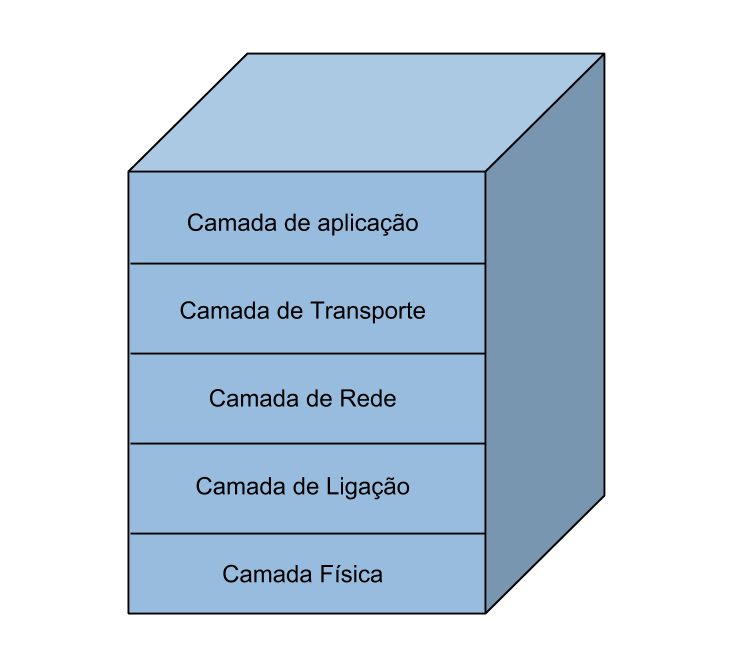
\includegraphics[width=230px,height=280px]{./Pictures/ProtocolStack.png}
% SensorNodesScatteredInASensorField.png: 816x1056 pixel, 96dpi, 21.59x27.94 cm, bb=0 0 612 792
% pdfLaTeX aceita figuras no formato PNG, JPG ou PDF
% figuras vetoriais podem ser exportadas para eps e depois convertidas para pdf usando epstopdf
\caption{Pilha de protocolos em redes de sensores sem fio} %legenda
\label{fig:protocolStack} %rotulo para refencia
\end{figure}


 %---------------------------------------------------------------------
 \subsubsection{Camada física (\textit{physical layer})} 
 %------------------------------------------------------

 A camada física é responsável por selecionar a frequência, geração de frequência portadora (\textit{carrier frequency generation}), detecção de sinais, modulação e encriptação de dados. O custo, tanto em termos de consumo de energia quanto em complexidade de implementação, da comunicação sem fio a longas distâncias é muito elevado. Em redes de sensores sem fio, a minimização do consumo de energia tem importância significativa na propagação e nos efeitos que causam desvanecimento do sinal. Em geral, a potência necessária para transmitir um sinal a uma distância \textit{$d$} é diretamente proporcional a \textit{$d^{n}$}, sendo 2 <= \textit{n} < 4. n é próximo de 4 para antenas muito baixas e canais muito próximas do chão \cite{Pottie2000}.
 
 %---------------------------------------------------------------------
 \subsubsection{Camada de ligação de dados (\textit{Data Link Layer}) }
 %--------------------------------------------------------------------
 
 Camada de ligação de dados é a camada responsável por multiplexação de fluxos de dados (\textit{data streams}), detecção de quadros de dados (\textit{data frames}), acesso ao meio (\textit{medium access}) e controle de erros (\textit{error control}).
 
 \subsubsection*{Protocolos de controle de acesso ao meio}
 
Os protocolos de controle de acesso ao meio (\textit{Medium Access Control Protocols}) são o foco desse trabalho e atuam nessa camada. Eles coordenam o acesso ao meio físico por nós ativos. Esses protocolos são de grande importância, uma vez que o canal de comunicação sem fio (\textit{wireless}) é inerentemente propenso a erros, além de outros problemas específicos desse tipo de rede, tais como: o problema do terminal escondido (\textit{hidden-terminal}), problema do terminal exposto (\textit{exposed-terminal}) e efeitos do desvanecimento de sinal (\textit{signal fading effects}) \cite{Kumar06mediumaccess}. Esses protocolos serão abordados mais detalhadamente na sessão ~\ref{sec:macProtocols}.

 
 %---------------------------------------------------------------------
 \subsubsection{Camada de rede (\textit{Network layer})} 
 %------------------------------------------------------
 
 Técnicas convencionais de roteamento não são aplicáveis às características específicas desse tipo de redes (abordadas na sessão~\ref{sec:featuresRSSF}). Segundo \citeauthoronline{Guerses2005} (\cite{Guerses2005}), os protocolos dessa camada são desenvolvidos com base nas seguintes restrições:
 
 \begin{itemize}
 \item \textbf{Não há um identificador global}, devido a existência de poucos dados de eventos e um grande número de nós.
 \item \textbf{Eficiência de energia} é necessária para aumentar o tempo de vida da rede.
 \item \textbf{Descoberta de rotas auto organizável} para lidar com mudanças na topologia da rede.
 \item \textbf{Modelo de distribuição de dados}, segundo \citeauthoronline{Tilak02ataxonomy} (\citeyear{Tilak02ataxonomy}), pode ser dos tipos:
 \subitem \textbf{contínuo} - sensores entregam os dados continuamente;
 \subitem \textbf{dirigido a eventos} - sensores entregam dados ao detectarem um evento de interesse;
 \subitem \textbf{dirigido a consultas} - os nós entregam dados a partir da uma solicitação iniciada pelo observador;
 \item \textbf{Processamento em rede} por meio da utilização de ``funções de agregação'' é um requisito para comunicação eficiente em termos de energia;
 \item \textbf{Comunicação local inter sensor} é um requisito para aplicações, bem como para o processamento em rede;
 \item \textbf{Qualidade de serviço} (largura de banda, quantidade de erros e latência) deve atender aos requisitos das aplicações; 
 
 \end{itemize}

 %---------------------------------------------------------------------
 \subsubsection{Camada de transporte (\emph{Transport Layer})} 
 %------------------------------------------------------
 
 Muitas aplicações de redes de sensores sem fio requerem mecanismos de controle de congestionamento para regular a quantidade de tráfego injetada na rede com o objetivo de evitar perda de pacotes e para atribuir confiabilidade à entrega de pacotes e eventos \cite{RaSaGu2008-InCol}. Em várias aplicações há nós responsáveis por capturar informações críticas e enviá-las a um nó concentrador (\textit{sink node}) \cite{RaSaGu2008-InCol}. Os protocolos dessa camada são desenvolvidos para atender a essas restrições e garantir que os pacotes sejam enviados e alcancem seus destinos corretamente.

 \subsubsection{Camada de aplicação (\emph{Application Layer})}
 
 Segundo \citeauthoronline{Akyildiz2002} (\citeyear{Akyildiz2002}), embora haja muitas aplicações propostas para redes de sensores, potenciais protocolos para a camada de aplicação permanecem em uma região altamente inexplorada. Esses protocolos possibilitam a interação entre a camada de aplicação e as camadas inferiores. Há três protocolos mais comuns utilizados nessa camada. 
 
 \begin{itemize}
 \item \textbf{Protocolo de gerenciamento de sensores:} protocolos de gerenciamento na camada de aplicação tornam o \textit{hardware} e o \textit{software} das camadas inferiores transparentes para aplicações de gerenciamento de redes de sensores.
 \item \textbf{Protocolo de atribuição de tarefas e anúncio de dados (\textit{data advertisement}):} utilizado para atribuição de tarefas aos nós e também para comunicação de detecção de eventos pelos nós.
 \item \textbf{Protocolo de requisição (\textit{sensor query}) e disseminação de dados:} utilizados para fazer consultas ou requisições de dados aos sensores e devolução das respectivas respostas.
 \end{itemize}